% Ceci est le dernier fichier TeX pour le cours de mathématiques financière.
% J'ai eu un problème d'encodage sur mon fichier principal, ce qui m'oblige à
% créer un dernier fichier pour le dernier cours qui va être indépendant!
\documentclass[12pt, french]{report}

% Préambule pour rédaction LaTeX

% Préparé par Gabriel Crépeault-Cauchon
% Si vous n'avez pas besoin de l'un des packages, simplement à indiquer un «%»
% au début
% -----------------------------------------------------------------------------

% Packages pour permettre les caractères accentués
\usepackage[utf8]{inputenc}
\usepackage[T1]{fontenc}
\usepackage{babel}
\usepackage{lmodern}

% Package pour aggrandir les marges d'un document
% \usepackage{fullpage}

% Packages mathématiques essentiels
\usepackage{amsmath,amsthm,amssymb,latexsym,amsfonts}
\usepackage{empheq}
\usepackage{numprint}


% Packages pour des graphiques avancés
\usepackage{graphicx}
\usepackage{pict2e}

% Package pour faire des listes plus avancées
\usepackage{enumitem}

% Packages pour créer des liens URL
\usepackage{hyperref}

% Package pour l'insertion de documents PDF à même un fichier LaTeX
\usepackage{pdfpages}

% Package pour éditer les couleurs du fichier
% \usepackage[svgnames]{xcolor}
\usepackage{color,soul}


% NOUVELLES COULEURS
\newcommand{\orange}{\textcolor{orange}}
\newcommand{\red}{\textcolor{red}}
\newcommand{\cyan}{\textcolor{cyan}}
\newcommand{\blue}{\textcolor{blue}}
\newcommand{\green}{\textcolor{green}}
\newcommand{\purple}{\textcolor{magenta}}
\newcommand{\yellow}{\textcolor{yellow}}


% Commandes pour certains symboles mathématiques...
\newcommand{\reels}{\mathbb{R}}
\newcommand{\entiers}{\mathbb{Z}}
\newcommand{\naturels}{\mathbb{N}}
\newcommand{\eval}{\biggr \rvert}
\usepackage{cancel}



% Package bclogo pour insérer des logos intéressant dans le fichier
\usepackage[tikz]{bclogo}
\usepackage{actuarialsymbol}
\usepackage{actuarialangle}

% Commandes utiles pour sauver du temps dans la rédaction
\newcommand{\p}{\paragraph{}}
\newcommand{\n}{\newline}



% Pr�sentation document
	\title{Notes du dernier cours \\ Mathématiques financières \\ Automne 2017 \\ ACT-1001}
	\author{Gabriel Crépeault-Cauchon}
	\date{Dernière mise à jour : \today}

% Mise en page du document
\usepackage{fancyhdr}
\pagestyle{fancy}
\fancyhead{}
\fancyhead[L]{\text{Dernier cours ACT-1001}}
\fancyhead[R]{\today}
\fancyfoot{}
\fancyfoot[RO,RE]{\thepage}
\renewcommand{\footrulewidth}{0.5pt}


% Commencer la numérotation des chapitres
\setcounter{chapter}{6}
% fin du pr�ambule


% ------------------------------------------------------------------------------
\begin{document}

% ------------------------------------------------------------------------------
\part*{Notes du dernier cours ACT-1001}


\chapter{Duration et immunisation}
\setcounter{section}{1}		% pour considérer les chapitres passés

\section{Appariement et immunisation}
Anglais :
\begin{itemize}
	\item Immunisation : \emph{Immunization}
	\item Appariement  : \emph{Asset-Liability matching (ALM)}
\end{itemize}
\p
Notation à utiliser :
\begin{itemize}
	\item $L_t$ : flux de passif (\emph{liabilities})
	\item $A_t$ : flux d'actif (\emph{assets})
\end{itemize}

\bcsmbh On suppose une structure plate ($s_0(t) = i \forall\ t$) et qu'on est
dans un marché efficient (on emprunte et investit au même taux).
\p
Objectif : on veut minimiser l'impact d'un changement dans le taux d'intérêt sur
la situation de la compagnie. On peut le faire par appariement, soit
\begin{displaymath}
	A_t = L_t \quad \forall\ t
\end{displaymath}
Dans le même sens,
\begin{displaymath}
	\sum_{t=0}^n (A_t - L_t)(1+i)^{-t} = 0
\end{displaymath}
Ce qui signifie qu'en changeant le taux d'intérêt, les $VA_A$ et $VA_L$ vont
changer, mais leur différence va toujours être égale à zéro. Nous en rediscuterons
dans la section sur l'immunisation complète (\ref{subsec:immunisation_complete}).
\p
Sans surprise,
\begin{equation}
	VA_A = \sum_{t=0}^n A_t(1+i)^{-t}
\end{equation}
\begin{equation}
	VA_L = \sum_{t=0}^n L_t(1+i)^{-t}
\end{equation}

\subsubsection*{Exemple}
On connaît $L_1 =1, \quad L_2 = 2, \quad L_3 = 3$. On veut savoir combien
d'obligations à coupon \emph{annuel} de 2\% il nous faut, selon leur échéance.
Les obligations sont notées $A_1, A_2$ et $A_3$, où $A_n$ est une obligation avec
échéance dans $n$ années. Pour les fins de l'exemple, on suppose un marché efficient
où l'on peut acheter des fractions d'obligations.
\p
On représente $\alpha_n$ comme le nombre d'obligation qui a échéance dans $n$ années.
\begin{align*}
	A_1	& = 2 \alpha_3		& + 2 \alpha_2			& + 102 \alpha_1			& = 1 \\
	A_2	& = 2 \alpha_3		& + 102 \alpha_2		& 										& = 1 \\
	A_3	& = 102 \alpha_3	& 									& 										& = 1 \\
\end{align*}
C'est un système d'équation très simple à résoudre en commencant par le flux d'actif $A_3$.


\subsection{Immunisation selon Redington}
\bcsmbh Encore une fois, cette section est dans un contexte de Structure plate.

\bcattention L'immunisation selon reddington fonctionne dans le cas où les taux
subissent un choc instantanée, mais que la structure reste néanmoins plate.
\begin{center}
	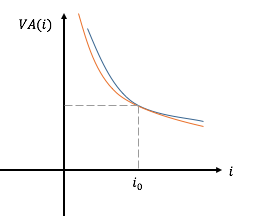
\includegraphics[width = 5cm, height = 5cm]{Reddington_graph.png}
\end{center}
Pour dire qu'on est immunisé, on désire que $VA_A > VA_L$ au taux actuel $i_0$ donné.
Toutefois, si on veut une immunisation totale en tout point, le flux d'actif doit
être plus convexe que le flux de passif. Bref, voici les 3 conditions de Redington
à respecter :

\begin{align}
	VA_A(i_0) 										& = VA_L(i_0) \\
	\frac{d}{di} VA_A	\eval_{i=i_0}			& = \frac{d}{di} VA_L \eval_{i = i_0} \\
	\frac{d^2}{di^2} VA_A \eval_{i=i_0}		& = \frac{d^2}{di^2} VA_L \eval_{i=i_0} \\
\end{align}
On peut ré-écrire ces 3 conditions de 2 autres façons :
\begin{align}
	VA_A(i_0) 				& = VA_L \\
	D_A(i_0)					& = D_L(i_0) \\
	C_A(i_0)					& = C_A(i_0) \\
\end{align}
\begin{align}
	VA_A(i_0) 				& = VA_L \\
	MD_A(i_0)					& = MD_L(i_0) \\
	MC_A(i_0)					& = MC_A(i_0) \\
\end{align}
\bcattention L'immunisation de Reddington ne fonctionne que pour un \underline{petit} choc.
\p
On pose donc les 2 premières conditions, puis on isole $A_{t_2}$ et $A_{t_2}$ Dans
les équations. Finalement, on valide la 3\up{e} condition pour la dérivée seconde.

\subsection{Immunisation complète}
\label{subsec:immunisation_complete}
en anglais : \emph{Full Immunization}.
\p
Définition : Les flux d'actifs immunisent complètement les flux de passif si
\begin{equation}
	VA_A(i) \ge VA_L(i) \quad \forall\ i >0
\end{equation}
\p
Remarque : l'immunisation, qu'elle soit complète ou selon Redington, requiert en
pratique des ajustements périodiques.
\p
La preuve mathématique a été faite en cours (je l'épargne ici) que si on a des
flux de passifs $L_t \quad t = r,r+1,...s-1,s$, ces derniers seront complètement
immunisés par des flux d'actifs $A_{t_1} \quad t_1 \le r$ et $A_{t_2} \quad t_2 \ge s$
si les 2 premières conditions de Redington sont respectées, soit
\begin{gather*}
	VA_A(i_0) = VA_L(i_0) \\
	t_1 A_{t_1}(1+i_0)^{-t_1} + t_2 A_{t_2} (1+i_0)^{-t_2} = \sum_{t=r}^s t L_t (1+i_0)^{-t} \\
\end{gather*}


% Fin du chapitre 7
\setcounter{chapter}{8}
\chapter{Sujets avancés en finance}
Dans le cadre du cours ACT-1001, on en voit qu'un seul : le modèle d'évaluation
des actions par l'actualisation des dividendes
\blue{(\href{https://www.investopedia.com/terms/d/ddm.asp}{Dividend Discount Model})}.

\section{Modèle d'évaluation des actions par l'actualisation des dividendes}
Tout d'abord, un peu de vocabulaire :
\begin{description}
	\item[Bid] cours acheteur (Prix offert le plus élevé) ;
	\item[Ask] cours vendeur (Prix demandé le plus faible) ;
	\item[Spread] écart acheteur-vendeur (différence entre le \emph{Bid} et le \emph{Ask}).
\end{description}
On a déjà vu les formules suivantes lorsqu'on a parlé de somme géométrique dans
le chapitre 2. $P$ est le prix de l'action, $d_t$ représente la dividende versé
au moment $t$ et $g$ représente le taux de croissance du dividende (s'il y a lieu).
\p
\subsection*{En présence d'une structure plate}

Si on a une structure plate ($i_t = i \forall\ t$) :
\begin{equation}
	P = \frac{d_1}{i - g}
\end{equation}

\subsection*{En présence d'une autre structure des taux}
Si on connaît nos taux au comptant (\emph{spot}):
\begin{equation}
	P = \sum_{t=1}^\infty d_t [1 + s_0(t)]^{-t}
\end{equation}

Si on connaît nos taux à terme (\emph{forward}) :
\begin{equation}
	P = \sum_{t=1}^\infty \prod_{u=1}^\infty \frac{d_t}{1 + i_0(u-1,u)}
\end{equation}







% ------------------------------------------------------------------------------
% Fin du document
\end{document}
% ------------------------------------------------------------------------------
